% %% file: template.tex = LaTeX template for article-like report 
%% init: sometime 1993
%% last: Feb  8 2015  Rob Rutten  Deil
%% site: http://www.staff.science.uu.nl/~rutte101/rrweb/rjr-edu/manuals/student-report/

%% First read ``latex-bibtex-simple-manual.txt'' at
%% http://www.staff.science.uu.nl/~rutte101/Report_recipe.html

%% Start your report production by copying this file into your XXXX.tex.
%% Small changes to the header part will make it an A&A or ApJ manuscript.

%%%%%%%%%%%%%%%%%%%%%%%%%%%%%%%%%%%%%%%%%%%%%%%%%%%%%%%%%%%%%%%%%%%%%%%%%%%%
%\documentclass{aa}   %% Astronomy & Astrophysics style class
\documentclass[a4paper]{report}
\usepackage[inner=2cm,outer=2cm]{geometry}
%\geometry{a4paper}
\usepackage{graphicx,url,twoopt}
\usepackage{subcaption}
\usepackage{enumitem}
\usepackage{amsmath}
\usepackage[varg]{txfonts}           %% A&A font choice
%\usepackage{hyperref}                %% for pdflatex
%%\usepackage[breaklinks]{hyperref}  %% for latex+dvips
%%\usepackage{breakurl}              %% for latex+dvips
%\usepackage{pdfcomment}              %% for popup acronym meanings
%\usepackage{acronym}                 %% for popup acronym meanings
\usepackage{calrsfs}
\DeclareMathAlphabet{\pazocal}{OMS}{zplm}{m}{n}

\usepackage{natbib}
% \hypersetup{
%   colorlinks=true,   %% links colored instead of frames
%   urlcolor=blue,     %% external hyperlinks
%   linkcolor=red,     %% internal latex links (eg Fig)
% }

 %\bibpunct{(}{)}{;}{a}{}{,}    %% natbib cite format used by A&A and ApJ
 
%\pagestyle{plain}   %% undo the fancy A&A pagestyle 


%%%%%%%%%%%%%%%%%%%%%%%%%%%%%%%%%%%%%%%%%%%%%%%%%%%%%%%%%%%%%%%%%%%%%%%%%%%%
\begin{document}  

%\twocolumn[{%
\vspace*{4ex}

\begin{center}
  {\Large \bf blablabla}\\[4ex]
  {\large \bf Andreas Ellewsen$^1$}\\[4ex]
  \begin{minipage}[t]{15cm}
        $^1$ Institute of Theoretical Astrophysics, University of Oslo, P.O. Box 1029 Blindern, N-0315 Oslo, Norway\\
             
        
    {\bf Abstract.} I compute the density perturbations, and velocities of dark matter and baryons. As well as the gravitational potentials $\Phi$ and $\Psi$. More importantly I also find $\Theta_0$.
    
  \vspace*{2ex}
  \end{minipage}
\end{center}
%}]
%\onecolumn
%%%%%%%%%%%%%%%%%%%%%%%%%%%%%%%%%%%%%%%%%%%%%%%%%%%%%%%%%%%%%%%%%%%%%%%%%%%%
\section{Introduction}\label{sec:introduction}
%%%%%%%%%%%%%%%%%%%%%%%%%%%%%%%%%%%%%%%%%%%%%%%%%%%%%%%%%%%%%%%%%%%%%%%%%%%%
In this project I will follow the algorithm presented in Callin (2005)[1] for simulating the cosmic microwave background.  
This is part three of four for this project.

In the first part I set up the background cosmology of the universe, and made a function that could find the conformal time as a function of $x$. In the second part I computed the electron fraction, electron density, optical depth and visibility function for times around and during recombination. 

In this part I will use some of these functions along with the Einstein-Boltzmann equations without polarization and neutrinos to compute the density perturbations, and velocities of dark matter and baryons. As well as the temperature multi poles $\Theta_l$.

As previously done I will continue building on the skeleton code provided.

%%%%%%%%%%%%%%%%%%%%%%%%%%%%%%%%%%%%%%%%%%%%%%%%%%%%%%%%%%%%%%%%%%%%%%%%%%%%
\section{Equations}\label{sec:Equations}
%%%%%%%%%%%%%%%%%%%%%%%%%%%%%%%%%%%%%%%%%%%%%%%%%%%%%%%%%%%%%%%%%%%%%%%%%%%%
The full set of Einstein-Boltzmann equations without polarization and neutrinos read
\begin{align}
 \Theta^\prime_0 =& -\frac{ck}{\pazocal{H}}\Theta_1 - \Phi^\prime\\
 \Theta^\prime_1 =& \frac{ck}{3\pazocal{H}}\Theta_0 - \frac{2ck}{3\pazocal{H}}\Psi + \tau^\prime\bigg[\Theta_1+\frac{1}{3}v_b\bigg]\\
 \Theta_l^\prime =& \frac{lck}{(2l+1)\pazocal{H}}\Theta_{l-1} - \frac{(l+1)ck}{(2l+1)\pazocal{H}}\Theta_{l+1} + \tau^\prime\bigg[\Theta_l-\frac{1}{10}\Theta_l\delta_{l,2} \bigg], 2\le l < l_{max}\\
 \Theta_l^\prime =& \frac{ck}{\pazocal{H}}\Theta_{l-1} - c\frac{l+1}{\pazocal{H}\eta(x)}\Theta_l + \tau^\prime\Theta_l, l=l_{max}\\
 \delta^\prime =&\frac{ck}{\pazocal{H}}v -3\Phi^\prime\\
 v^\prime =& -v -\frac{ck}{\pazocal{H}}\Psi\\
 \delta^\prime_b =& \frac{ck}{\pazocal{H}}v_b - 3\Phi^\prime\\
 v_b^\prime =& -v_b - \frac{ck}{\pazocal{H}}\Psi +\tau^\prime R(3\Theta_1+v_b)\\
 \Phi^\prime =& \Psi - \frac{c^2 k^2}{3\pazocal{H}^2}\Phi + \frac{H_0^2}{2\pazocal{H}^2}\bigg[\Omega_m a^{-1}\delta + \Omega_b a^{-1}\delta_b +4\Omega_r a^{-2}\Theta_0 \bigg]\\
 R =& \frac{4\Omega_r}{3\Omega_b a}.
\end{align}

These equations are the ones we will use when we are not in the tight coupling regime. When in the tight coupling regime the factor $(3\Theta_1+v_b)$ is very close to zero. In the equation for $v_b^\prime$ this is multiplied by $\tau^\prime$ which is very large in, making this equation terribly unstable. The same thing makes the equation for $\Theta^\prime_1$ unstable. Because of this one expand $(3\Theta_1+v_b)$ in powers of $1/tau^\prime$. This results in 
a slight change in the set of equations for $v_b^\prime$ and $\Theta_l$.

\begin{align} 
q &= \frac{-[(1-2R)\tau^\prime + (1+R)\tau^{\prime\prime}](3\Theta_1+v_b) - \frac{ck}{\pazocal{H}}\Psi + (1-\frac{\pazocal{H}^\prime}{\pazocal{H}})\frac{ck}{\pazocal{H}}(-\Theta_0+2\Theta_2) - \frac{ck}{\pazocal{H}}\Theta_0^\prime} {(1+R)\tau^\prime + \frac{\pazocal{H}^\prime}{\pazocal{H}} - 1}\\
v_b^\prime &= \frac{1}{1+R}\bigg[ -v_b - \frac{ck}{\pazocal{H}}\Psi + R(q + \frac{ck}{\pazocal{H}}(-\Theta_0+2\Theta_2)-\frac{ck}{\pazocal{H}}\Psi) \bigg]\\
\Theta_1^\prime &= \frac{1}{3}(q - v_b^\prime).
 \end{align}

So far I have not stated what tight coupling means. Basically because of the mathematical operations we have done, like expanding in powers of $1/tau^\prime$, we end up with some conditions on when these equations above can be used. The conditions are $|ck/(\pazocal{H}\tau^\prime)| < 1/10$, $|\tau^\prime|>10$, and that the time is before recombination.
 
All of these equations refer to their respective quantities in Fourier space. This means that the $k$'s everywhere refer to Fourier modes. This is done to separate the quantities into the different scales at which they take place, with low $k$'s referring to large scales, and high $k$'s to small scales.
 
%%%%%%%%%%%%%%%%%%%%%%%%%%%%%%%%%%%%%%%%%%%%%%%%%%%%%%%%%%%%%%%%%%%%%%%%%%%%
\section{Implementation}\label{sec:Imp}
%%%%%%%%%%%%%%%%%%%%%%%%%%%%%%%%%%%%%%%%%%%%%%%%%%%%%%%%%%%%%%%%%%%%%%%%%%%%
The way to solve all these equations is to first make a function that finds the time where tight coupling ends.
Note that this function clearly depends on which k mode we are working on.

For each k we insert the initial conditions, and then run through every value of x from some start value early in the universe. In this case I have chosen to use the $x$ value corresponding to $a_{init} = 10^{-8}$.
At some point through this the $x$ value becomes larger than the $x$ at the end of tight coupling. At that point we change the equations for the relevant quantities, and continue on until we reach today.
This has to be done for all k values. I have chosen to set the limit at $k=100$ so far. With this low k value the program completes in less than five minutes.

It should also be said that we limit our number of $l$'s to six. This can be done because we are using line of sight integration. Historically people used to include thousands of variables to trace multi poles. If we had to use this the program would use days or weeks instead of minutes.

%%%%%%%%%%%%%%%%%%%%%%%%%%%%%%%%%%%%%%%%%%%%%%%%%%%%%%%%%%%%%%%%%%%%%%%%%%%%
\section{Results}\label{sec:results}
%%%%%%%%%%%%%%%%%%%%%%%%%%%%%%%%%%%%%%%%%%%%%%%%%%%%%%%%%%%%%%%%%%%%%%%%%%%%
To get a good distribution of k modes we use a quadratic distribution in k such that
\begin{equation}
 k_i = k_{min} +(k_{max}-k_{min})(i/100)^2,
\end{equation}
where $k_{max} = 1000H_0/c$, and $k_{min} = 0.1H_0/c$.
The results show the various quantities for six different k values. These k values are $k_1,k_5,k_{10},k_{40},k_{60},k_{100}$. 

\begin{figure}
\begin{subfigure}{.5\textwidth}
  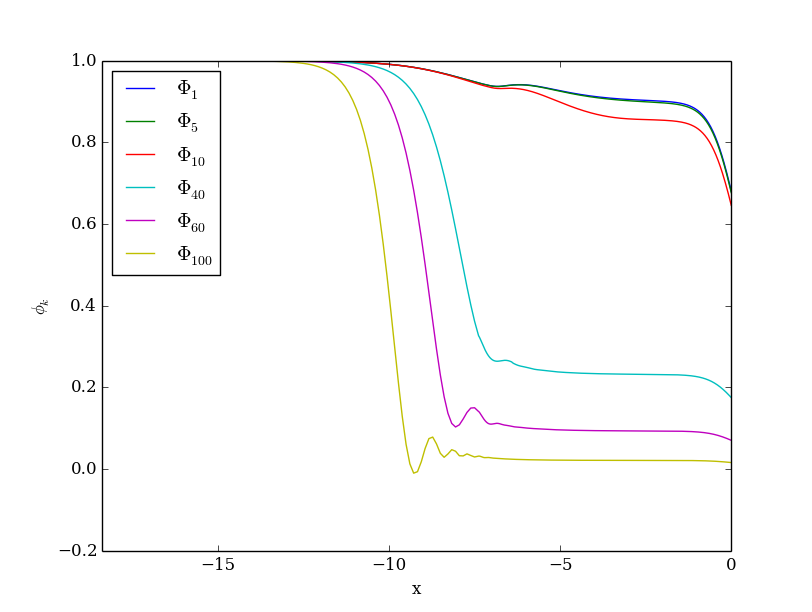
\includegraphics[width=\textwidth]{Phi.png}
 \caption{The plot for $\Phi$ for six different k's.}
 \label{fig:Phi}
\end{subfigure}
\begin{subfigure}{.5\textwidth}
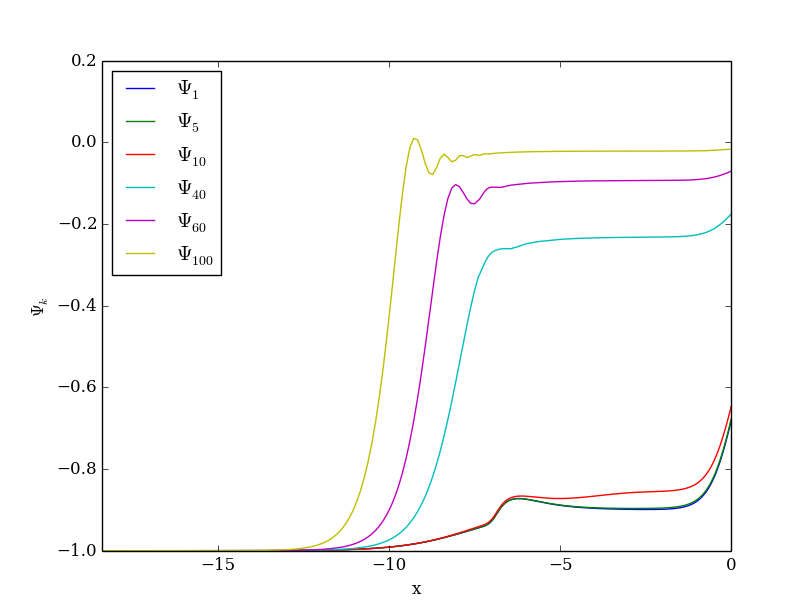
\includegraphics[width=\textwidth]{Psi.png}
 \caption{The plot for $\Psi$ for six different k's.}
 \label{fig:Psi}
\end{subfigure}
\caption{The first thing to note is that the plots seem to be the inverse of each other. Also all the modes of $\Phi$ start at 1, and decrease as they leave tight coupling. The higher the mode, the closer to 0 they stabilize after recombination. The higher modes oscillate a bit before stabilizing around recombination. This is not seen in the lower modes. The smallest modes do not show this oscillating behavior at all, instead they slowly decrease after tight coupling before doing a nose dive near the end. The behavior of $\Psi$ is the complete inverse of this.}
\end{figure}

\begin{figure}
\begin{subfigure}{.5\textwidth}
  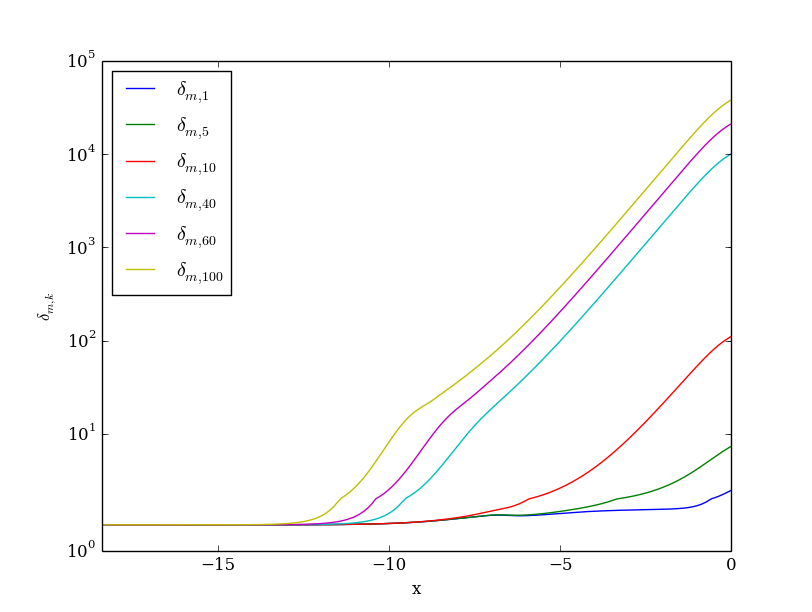
\includegraphics[width=\textwidth]{delta.png}
 \caption{The plot for $\delta$ for six different k's.}
 \label{fig:delta}
\end{subfigure}
\begin{subfigure}{.5\textwidth}
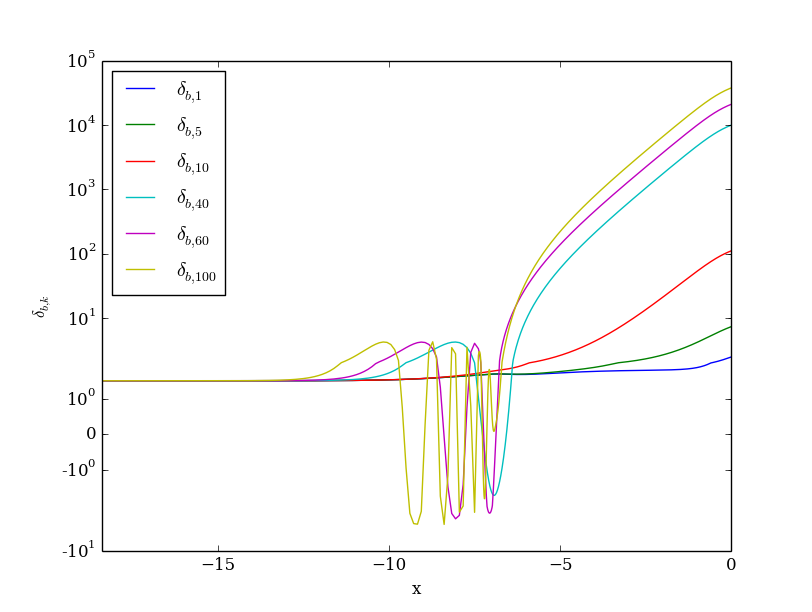
\includegraphics[width=\textwidth]{deltab.png}
 \caption{The plot for $\delta_b$ for six different k's.}
 \label{fig:deltab}
\end{subfigure}
\caption{Note the special y axis on the plot for $\delta_b$. The dark matter perturbations behave nicely. The higher the mode the earlier it can start growing, just as expected due to the fact that forces don't propagate instantaneously. Note also that all the dark matter perturbations remain positive. This is not the case for baryons. When we start approaching recombination all the higher order modes start oscillating, and it is only after recombination is done that they are allowed to start growing again, and now the can behave like dark matter.}
\end{figure}

\begin{figure}
\begin{subfigure}{.5\textwidth}
  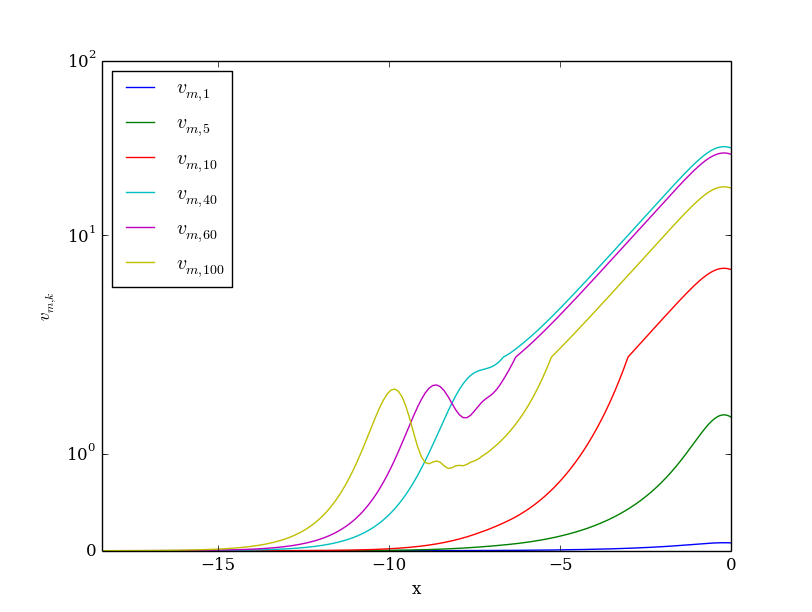
\includegraphics[width=\textwidth]{v.png}
 \caption{The plot for $v$ for six different k's.}
 \label{fig:v}
\end{subfigure}
\begin{subfigure}{.5\textwidth}
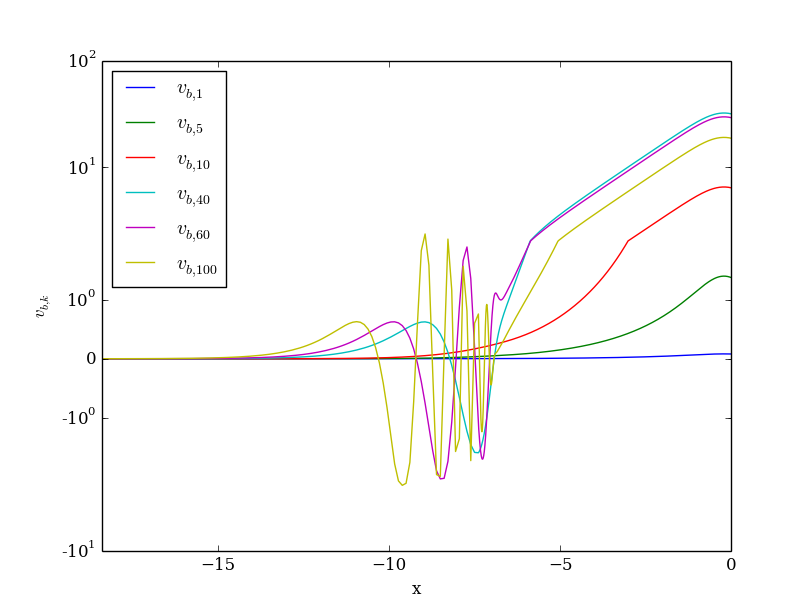
\includegraphics[width=\textwidth]{vb.png}
 \caption{The plot for $v_b$ for six different k's.}
 \label{fig:vb}
\end{subfigure}
\caption{As before there is a clear difference between the velocities of the two components. The highest modes start growing first, and since they are larger when approaching recombination they slow down more. Note the yellow and purple curves in the $v$ plot. The lower modes don't slow down, but they don't increase as fast, while the smallest modes don't notice anything special happening. The velocity of the baryons is very different. As the dark matter, the highest modes start growing first, but as they exit tight coupling they start to oscillate, expanding and contracting, until after recombination where they speed up again to catch up with the dark matter. Note that the lowest modes don't notice anything special happening here either. In fact, they are fairly equal for dark matter and baryons.}
\end{figure}

\begin{figure}
 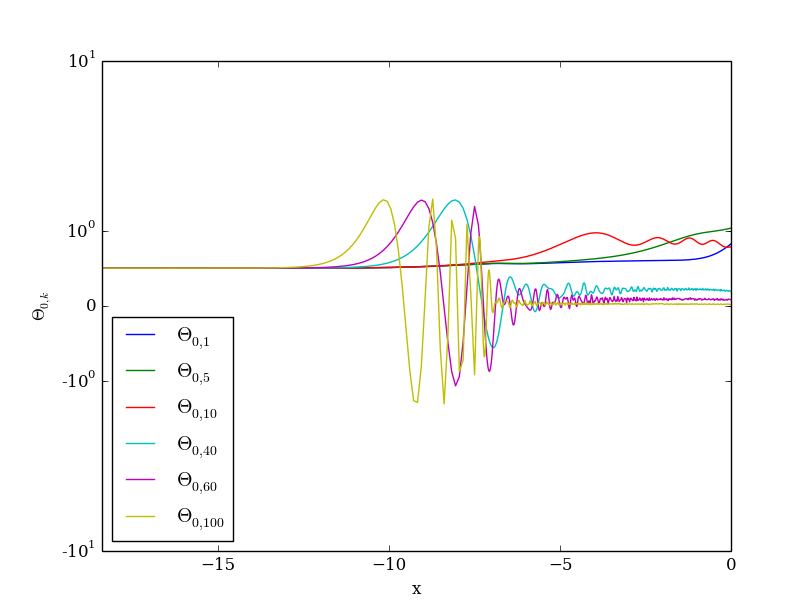
\includegraphics[width=\textwidth]{Theta0.png}
 \caption{The plot shows $\Theta_0$ for six different k's. The low modes stay constant until the time at which their corresponding baryon perturbations start growing. This is as expected since $\Theta_0$ measures the mean temperature, and this should increases as baryons clump together because of gravity. The high modes oscillate like their corresponding perturbation modes do. However, they do not grow after recombination, instead they stabilize around values fairly close to zero. The intermediate modes like $k_{10}$ oscillate around some value between 0.5 and 1.}
 \label{fig:Theta0}
\end{figure}





%%%%%%%%%%%%%%%%%%%%%%%%%%%%%%%%%%%%%%%%%%%%%%%%%%%%%%%%%%%%%%%%%%%%%%%%%%%%
\section{Conclusions} \label{sec:conclusions}
%%%%%%%%%%%%%%%%%%%%%%%%%%%%%%%%%%%%%%%%%%%%%%%%%%%%%%%%%%%%%%%%%%%%%%%%%%%%
We have calculated the density perturbations and velocities of dark matter and baryons. We also found the gravitational potentials $\Psi$ and $\Phi$. And most importantly we found the evolution of the temperature multi poles $\Theta_l$ which will enable us to make a map of the cosmic microwave background in the next and final part of the project.
%%%%%%%%%%%%%%%%%%%%%%%%%%%%%%%%%%%%%%%%%%%%%%%%%%%%%%%%%%%%%%%%%%%%%%%%%%%%
\section{References}
%%%%%%%%%%%%%%%%%%%%%%%%%%%%%%%%%%%%%%%%%%%%%%%%%%%%%%%%%%%%%%%%%%%%%%%%%%%%
\begin{enumerate}[label= {[}\arabic*{]} ]
 \item P. Callin, astro-ph/0606683
\end{enumerate}

\onecolumn 
%%%%%%%%%%%%%%%%%%%%%%%%%%%%%%%%%%%%%%%%%%%%%%%%%%%%%%%%%%%%%%%%%%%%%%%%%%%%
\section{Source code}\label{sec:files}
%%%%%%%%%%%%%%%%%%%%%%%%%%%%%%%%%%%%%%%%%%%%%%%%%%%%%%%%%%%%%%%%%%%%%%%%%%%%
The source code for the evolution\_mod file is included for inspection. This file depends on all files previously used in the two earlier parts of the project.

\begin{verbatim}
 module evolution_mod
  use healpix_types
  use params
  use time_mod
  use ode_solver
  use rec_mod
  implicit none

  !Use j,k,l as global variable
  integer(i4b) :: j,k,l

  ! Accuracy parameters
  real(dp),     parameter, private :: k_min    = 0.1d0 * H_0 / c
  real(dp),     parameter, private :: k_max    = 1.d3  * H_0 / c
  integer(i4b), parameter          :: n_k      = 100
  integer(i4b), parameter, private :: lmax_int = 6

  ! Perturbation quantities
  real(dp), allocatable, dimension(:,:,:) :: Theta
  real(dp), allocatable, dimension(:,:)   :: delta
  real(dp), allocatable, dimension(:,:)   :: delta_b
  real(dp), allocatable, dimension(:,:)   :: Phi
  real(dp), allocatable, dimension(:,:)   :: Psi
  real(dp), allocatable, dimension(:,:)   :: v
  real(dp), allocatable, dimension(:,:)   :: v_b
  real(dp), allocatable, dimension(:,:)   :: dPhi
  real(dp), allocatable, dimension(:,:)   :: dPsi
  real(dp), allocatable, dimension(:,:)   :: dv_b
  real(dp), allocatable, dimension(:,:,:) :: dTheta

  real(dp), allocatable, dimension(:) :: dtau
  real(dp), allocatable, dimension(:) :: ddtau
  real(dp), allocatable, dimension(:) :: H_p
  real(dp), allocatable, dimension(:) :: dH_p
  real(dp), allocatable, dimension(:),private :: eta_precomp

  ! Fourier mode list
  real(dp), allocatable, dimension(:) :: ks

  ! Book-keeping variables
  real(dp),     private :: k_current,ck_current,ckH_p
  integer(i4b), private :: npar = 6+lmax_int

  !With or without polarization
  !logical(lgt) :: polarize = False
contains


  ! NB!!! New routine for 4th milestone only; disregard until then!!!
  !subroutine get_hires_source_function(k, x, S)
  !  implicit none

  !  real(dp), pointer, dimension(:),   intent(out) :: k, x
  !  real(dp), pointer, dimension(:,:), intent(out) :: S

  !   integer(i4b) :: i, j
  !  real(dp)     :: g, dg, ddg, tau, dt, ddt, H_p, dH_p, ddHH_p, Pi, dPi, ddPi
  !  real(dp), allocatable, dimension(:,:) :: S_lores

    ! Task: Output a pre-computed 2D array (over k and x) for the 
    !       source function, S(k,x). Remember to set up (and allocate) output 
    !       k and x arrays too. 
    !
    ! Substeps:
    !   1) First compute the source function over the existing k and x
    !      grids
    !   2) Then spline this function with a 2D spline
    !   3) Finally, resample the source function on a high-resolution uniform
    !      5000 x 5000 grid and return this, together with corresponding
    !      high-resolution k and x arrays

 ! end subroutine get_hires_source_function


  ! Routine for initializing and solving the Boltzmann and Einstein equations
  subroutine initialize_perturbation_eqns
    implicit none
    integer(i4b) :: i
    real(dp)     :: k_min = 0.1d0*H_0/c
    real(dp)     :: k_max = 1000.d0*H_0/c

    !Initialize k-grid, ks; quadratic between k_min and k_max
    allocate(ks(n_k))
    do k=1,n_k
        ks(k) = k_min +(k_max -k_min)*((k-1)/100.d0)**2
    end do

    !Allocate arrays for perturbation quantities
    allocate(delta(1:n_t, n_k))
    allocate(delta_b(1:n_t, n_k))
    allocate(v(1:n_t, n_k))
    allocate(v_b(1:n_t, n_k))
    allocate(Phi(1:n_t, n_k))
    allocate(Theta(1:n_t, 0:lmax_int, n_k))
    allocate(Psi(1:n_t, n_k))

    allocate(dPhi(1:n_t, n_k))
    allocate(dPsi(1:n_t, n_k))
    allocate(dv_b(1:n_t, n_k))
    allocate(dTheta(1:n_t, 0:lmax_int, n_k))

    !Allocate arrays for precomputed variables
    allocate(dtau(n_t),H_p(n_t),dH_p(n_t))
    allocate(ddtau(n_t),eta_precomp(n_t))

    !Precompute useful variables
    do i=1,n_t
       dtau(i)  = get_dtau(x_t(i))
       ddtau(i) = get_ddtau(x_t(i))
       H_p(i)   = get_H_p(x_t(i))
       dH_p(i)  = get_dH_p(x_t(i))
       eta_precomp(i)   = get_eta(x_t(i))
    end do
    write(*,'(*(2X, ES14.6))') H_p(1),dH_p(1),ddtau(1),dtau(1),ks(1)
    ! Task: Set up initial conditions for the Boltzmann and Einstein equations
    Phi(1,:)     = 1.d0
    delta(1,:)   = 1.5d0*Phi(1,:)
    delta_b(1,:) = delta(1,:)
    Theta(1,0,:) = 0.5d0*Phi(1,:)
    do k = 1, n_k
        v(1,k)       = c*ks(k)/(2.d0*H_p(1))*Phi(1,k)
        v_b(1,k)     = v(1,k)
        Theta(1,1,k) = -c*ks(k)/(6.d0*H_p(1))*Phi(1,k)
        Theta(1,2,k) = -20.d0*c*ks(k)/(45.d0*H_p(1)*dtau(1))*Theta(1,1,k) !without polarization
        do l = 3, lmax_int
            Theta(1,l,k) = -l/(2.d0*l+1.d0)*c*ks(k)/(H_p(1)*dtau(1))*Theta(1,l-1,k)
        end do
        Psi(1,k)     = -Phi(1,k) - 12.d0*H_0**2/(ks(k)*c*a_t(1))**2*Omega_r*Theta(1,2,k)
    end do
  end subroutine initialize_perturbation_eqns

  subroutine integrate_perturbation_eqns
    implicit none
    real(dp)     :: x1, x2, x_init
    real(dp)     :: eps, hmin, h1, x_tc, j_tc, dt, t1, t2
    real(dp)     :: R,d_v,d_v_b,q
    real(dp), allocatable, dimension(:) :: y, y_tight_coupling, dydx
    eps    = 1.d-8
    hmin   = 0.d0
    h1     = 1.d-5
    allocate(y(npar))
    allocate(dydx(npar))
    allocate(y_tight_coupling(7))

    dydx(:) = 0

    ! Propagate each k-mode independently
    do k = 1, n_k
       write(*,*) 'Current k', k
       k_current = ks(k)  ! Store k_current as a global module variable
       ck_current = c*ks(k) !store c*k

       ! Initialize equation set for tight coupling
       y_tight_coupling(1) = delta(1,k)
       y_tight_coupling(2) = delta_b(1,k)
       y_tight_coupling(3) = v(1,k)
       y_tight_coupling(4) = v_b(1,k)
       y_tight_coupling(5) = Phi(1,k)
       y_tight_coupling(6) = Theta(1,0,k)
       y_tight_coupling(7) = Theta(1,1,k)
       
       ! Find the time to which tight coupling is assumed, 
       ! and integrate equations to that time
       x_tc = get_tight_coupling_time(k_current)
       !write(*,*) 'x_tc =',x_tc
       !write(*,*) 'under x_tc'

       ! Task: Integrate from x_init until the end of tight coupling, using
       !       the tight coupling equations
       !write(*,*) 'Start of tight coupling'
       !write (*,'(*(2X, ES14.6))') delta(1,k), delta_b(1,k), v(1,k), v_b(1,k), Phi(1,k), Theta(1,0,k), Theta(1,1,k),Psi(1,k)
       !write (*,'(*(2X, ES14.6))') x_t(1),dv_b(1,k),dPsi(1,k),dPhi(1,k),dTheta(1,0,k),dTheta(1,1,k),dTheta(1,2,k)

       do j=2,n_t
           if (x_t(j)< x_tc) then 
               !precompute some variables
               ckH_p = ck_current/H_p(j)

               !Solve next step
               call odeint(y_tight_coupling,x_t(j-1),x_t(j),eps,h1,hmin,derivs_tc, bsstep, output3)

               !Save variables
               delta(j,k)   = y_tight_coupling(1)
               delta_b(j,k) = y_tight_coupling(2)
               v(j,k)       = y_tight_coupling(3)
               v_b(j,k)     = y_tight_coupling(4)
               Phi(j,k)     = y_tight_coupling(5)
               Theta(j,0,k) = y_tight_coupling(6)
               Theta(j,1,k) = y_tight_coupling(7)
               Theta(j,2,k) = -(20.d0*ckH_p)/(45.d0*dtau(j))*Theta(j,1,k)
               do l = 3, lmax_int
                  Theta(j,l,k) = -l/(2.d0*l+1.d0)*ckH_p/dtau(j)*Theta(j,l-1,k)
               end do	
               Psi(j,k)      = -Phi(j,k) - 12.d0*H_0**2/(ck_current*a_t(j))**2*Omega_r*Theta(j,2,k)

               !Store derivatives that are required for C_l estimation
               dPhi(j,k)     = Psi(j,k) - (ckH_p)**2/3.d0*Phi(j,k) + (H_0**2/H_p(j))**2/2.d0 &
                              *(Omega_m/a_t(j)*delta(j,k) + Omega_b/a_t(j)*delta_b(j,k) &
                              + 4.d0*Omega_r/a_t(j)**2 *Theta(j,0,k))

               dPsi(j,k)     = -dPhi(j,k) - 12.d0*H_0**2/(ck_current*a_t(j))**2*Omega_r*(-2.d0*Theta(j,2,k)+dTheta(j,2,k))

               dTheta(j,0,k) = -ckH_p*Theta(j,1,k) - dPhi(j,k)

               R             = 4.d0*Omega_r/(3.d0*Omega_b*a_t(j))

               q             = (-((1.d0-2.d0*R)*dtau(j) + &
                              (1.d0+R)*ddtau(j))*(3.d0*Theta(j,1,k)+v_b(j,k)) - &
                              ckH_p*Psi(j,k) +&
                              (1.d0-dH_p(j)/H_p(j))*ckH_p*(-Theta(j,0,k) + 2.d0*Theta(j,2,k))-&
                              ckH_p*dTheta(j,0,k))/((1.d0+R)*dtau(j)+dH_p(j)/H_p(j) -1.d0)
 
               dv_b(j,k)     = 1.d0/(1.d0+R)*(-v_b(j,k)-ckH_p*Psi(j,k)+&
                              R*(q+ckH_p*(2.d0*Theta(j,2,k)-Theta(j,0,k))-&
                              ckH_p*Psi(j,k)))

               dTheta(j,1,k) = 1.d0/3.d0*(q-dv_b(j,k))
               dTheta(j,2,k) = 0
               do l = 3, lmax_int
                   dTheta(j,l,k) = 0 
               end do	

               !write (*,'(*(2X, ES14.6))') delta(j,k), delta_b(j,k), v(j,k), v_b(j,k), Phi(j,k),  Theta(j,0,k), Theta(j,1,k),Psi(j,k)
               !write (*,'(*(2X, ES14.6))') x_t(j),dPsi(j,k),dPhi(j,k),dv_b(j,k),dTheta(j,0,k),dTheta(j,1,k),dTheta(j,2,k)


           else
               j_tc = j
               exit
           end if
       end do
       !write(*,*) 'End of tight coupling'

       ! Task: Set up variables for integration from the end of tight coupling 
       ! until today
       y(1:7) = y_tight_coupling(1:7)
       y(8)   = Theta(1,2,k)
       do l = 3, lmax_int
          y(6+l) = Theta(1,l,k)
       end do


       !Continue after tight coupling
       !write(*,*) 'start of rec'       
       do j = j_tc, n_t

          !Precompute some variables
          ckH_p = ck_current/H_p(j)

          !Integrate equations from tight coupling to today
          !write(*,*) 'running odeint with j =', j
          call odeint(y, x_t(j-1) ,x_t(j), eps, h1, hmin, derivs, bsstep, output3)

          ! Task: Store variables at time step i in global variables
          delta(j,k)   = y(1)
          delta_b(j,k) = y(2)
          v(j,k)       = y(3)
          v_b(j,k)     = y(4)
          Phi(j,k)     = y(5)
          
          do l = 0, lmax_int
             Theta(j,l,k) = y(6+l)
          end do
          Psi(j,k)     =  - Phi(j,k) - 12.d0*H_0**2/(ck_current*a_t(j))**2*Omega_r*Theta(j,2,k)

          ! Task: Store derivatives that are required for C_l estimation
          dPhi(j,k)     = Psi(j,k) -c**2*k_current**2/(3.d0*H_p(j)**2)*Phi(j,k) +H_0**2/(2.d0*H_p(j)) &
                          *(Omega_m/a_t(j)*delta(j,k) +Omega_b/a_t(j)*delta_b(j,k) + 4.d0*Omega_r/a_t(j)**2 &
                          *Theta(j,0,k))

          dv_b(j,k)     = -v_b(j,k) -ckH_p*Psi(j,k) +dtau(j)*R*(3.d0*Theta(j,1,k)+ v_b(j,k))

          dTheta(j,0,k) = -ckH_p*Theta(j,1,k) -dPhi(j,k)
          dTheta(j,1,k) = ckH_p/3.d0*Theta(j,0,k) - &
                          2.d0*ckH_p/3.d0*Theta(j,2,k)+&
                          ckH_p/3.d0*Psi(j,k) + &
                          dtau(j)*(Theta(j,1,k)+ 1.d0/3.d0*v_b(j,k))
          dTheta(j,2,k) = 2.d0*ckH_p/5.d0*Theta(j,1,k) -&
                          3.d0*ckH_p/5.d0*Theta(j,3,k)+&
                          dtau(j)*0.9d0*Theta(j,2,k)
          do l=3,lmax_int-1
              dTheta(j,l,k) = l*ckH_p/(2.d0*l+1.d0)*Theta(j,l-1,k) -&
                              (l+1.d0)*ckH_p/(2.d0*l+1.d0)*Theta(j,l+1,k)+&
                              dtau(j)*Theta(j,l,k)
          end do
          dTheta(j,lmax_int,k) = ckH_p*Theta(j,l-1,k) -&
                                 c*(l+1.d0)/(H_p(j)*eta_precomp(j))*&
                                 Theta(j,l,k) + dtau(j)*Theta(j,l,k)
          dPsi(j,k)     = -dPhi(j,k) - 12.d0*H_0**2/(ck_current*a_t(j))**2*Omega_r*(-2.d0*Theta(j,2,k)+dTheta(j,2,k))
       end do
       !write(*,*) 'today'
    end do
    deallocate(y_tight_coupling)
    deallocate(y)
    deallocate(dydx)

  end subroutine integrate_perturbation_eqns

  subroutine derivs_tc(x,y_tc, dydx)
      use healpix_types
      implicit none
      real(dp),               intent(in)  :: x
      real(dp), dimension(:), intent(in)  :: y_tc
      real(dp), dimension(:), intent(out) :: dydx

      real(dp) :: d_delta
      real(dp) :: d_delta_b
      real(dp) :: d_v
      real(dp) :: q,R

      real(dp) :: delta,delta_b,v,v_b,Phi,Theta0,Theta1,Theta2
      real(dp) :: Psi,dPhi,dTheta0,dv_b,dTheta1

      delta   = y_tc(1)
      delta_b = y_tc(2)
      v       = y_tc(3)
      v_b     = y_tc(4)
      Phi     = y_tc(5)
      Theta0  = y_tc(6)
      Theta1  = y_tc(7)

      Theta2    = -20.d0*ckH_p/(45.d0*dtau(j))*Theta1

      R         = (4.d0*Omega_r)/(3.d0*Omega_b*a_t(j))

      Psi       = -Phi - 12.d0*(H_0/ck_current/a_t(j))**2.d0*Omega_r*Theta2

      dPhi      = Psi - ckH_p**2/3.d0*Phi + (H_0/H_p(j))**2/2.d0*(Omega_m/a_t(j)*delta + Omega_b/a_t(j)*delta_b + 4.d0*Omega_r/a_t(j)**2*Theta0)

      dTheta0   = -ckH_p*Theta1 - dPhi

      d_delta   = ckH_p*v   - 3.d0*dPhi

      d_delta_b = ckH_p*v_b - 3.d0*dPhi

      d_v       = -v -ckH_p*Psi

      q         = ( -((1.d0-2.d0*R)*dtau(j) + (1.d0+R)*ddtau(j)) *(3.d0*Theta1+v_b) - ckH_p*Psi +(1.d0-dH_p(j)/H_p(j))*ckH_p*(-Theta0 + 2.d0*Theta2) - ckH_p*dTheta0) / ((1.d0+R)*dtau(j)+dH_p(j)/H_p(j) -1.d0)

      dv_b      = (1.d0/(1.d0+R)) *(-v_b - ckH_p*Psi + R*(q+ckH_p*(-Theta0 + 2.d0*Theta2)-ckH_p*Psi))

      dTheta1   = (1.d0/3.d0)*(q-dv_b)

      dydx(1) = d_delta
      dydx(2) = d_delta_b
      dydx(3) = d_v
      dydx(4) = dv_b
      dydx(5) = dPhi
      dydx(6) = dTheta0
      dydx(7) = dTheta1
      !write(*,*) 'dydx(1) =',dydx(1)
      !write(*,*) 'dydx(2) =',dydx(2)
  end subroutine derivs_tc

  subroutine derivs(x,y, dydx) 
      use healpix_types
      implicit none
      real(dp),               intent(in)  :: x
      real(dp), dimension(:), intent(in)  :: y
      real(dp), dimension(:), intent(out) :: dydx

      real(dp) :: d_delta
      real(dp) :: d_delta_b
      real(dp) :: d_v
      real(dp) :: q,R
      integer(i4b) :: i
      real(dp) :: delta,delta_b,v,v_b,Phi,Theta0,Theta1,Theta2,Theta3,Theta4,Theta5,Theta6
      real(dp) :: Psi,dPhi,dTheta0,dv_b,dTheta1,dTheta2

      delta   = y(1)
      delta_b = y(2)
      v       = y(3)
      v_b     = y(4)
      Phi     = y(5)
      Theta0  = y(6)
      Theta1  = y(7)
      Theta2  = y(8)
      Theta3  = y(9)
      Theta4  = y(10)
      Theta5  = y(11)
      Theta6  = y(12)

      R         = (4.d0*Omega_r)/(3.d0*Omega_b*a_t(j))

      Psi       = -Phi - 12.d0*(H_0/ck_current/a_t(j))**2.d0*Omega_r*Theta2

      dPhi      = Psi - ckH_p**2/3.d0*Phi + (H_0/H_p(j))**2/2.d0*(Omega_m/a_t(j)*delta + Omega_b/a_t(j)*delta_b + 4.d0*Omega_r/a_t(j)**2*Theta0)

      dTheta0   = -ckH_p*Theta1 - dPhi

      d_delta   = ckH_p*v   - 3.d0*dPhi

      d_delta_b = ckH_p*v_b - 3.d0*dPhi

      d_v       = -v -ckH_p*Psi

      dv_b      = -v_b -ckH_p*Psi +dtau(j)*R*(3.d0*Theta1+v_b)

      dTheta1   = ckH_p/3.d0*Theta0 -2.d0/3.d0*ckH_p*Theta2 +ckH_p/3.d0*Psi +dtau(j)*(Theta1+v_b/3.d0)
      dTheta2   = l/(2.d0*l+1)*ckH_p*Theta1 - (l+1.d0)/(2.d0*l+1.d0)*ckH_p*Theta3+dtau(j)*0.9d0*Theta2

      do i=3,lmax_int-1
          dydx(6+i) = l/(2.d0*l+1)*ckH_p*y(5+i) - (l+1.d0)/(2.d0*l+1.d0)*ckH_p*y(7+i) +dtau(j)*y(6+i)
      end do

      dydx(12) = ckH_p*Theta5 -c*(l+1.d0)/H_p(j)/eta_precomp(j)*Theta6 +dtau(j)*Theta6

      dydx(1) = d_delta
      dydx(2) = d_delta_b
      dydx(3) = d_v
      dydx(4) = dv_b
      dydx(5) = dPhi
      dydx(6) = dTheta0
      dydx(7) = dTheta1
      dydx(8) = dTheta2
      !write(*,*) 'dydx(1) =',dydx(1)
      !write(*,*) 'dydx(2) =',dydx(2)
  end subroutine derivs

  subroutine output3(x, y)
      use healpix_types
      implicit none
      real(dp),               intent(in)  :: x
      real(dp), dimension(:), intent(in)  :: y
  end subroutine output3


  ! Task: Complete the following routine, such that it returns the time at which
  !       tight coupling ends. In this project, we define this as either when
  !       dtau < 10 or c*k/(H_p*dt) > 0.1 or x > x(start of recombination)
  function get_tight_coupling_time(k)
    implicit none

    real(dp), intent(in)  :: k
    real(dp)              :: get_tight_coupling_time
    integer(i4b)          :: i,n
    real(dp)              :: x
    n =1d4
    do i=0,n
        x = x_init +i*(0.d0-x_init)/n
        !write(*,*) x,x_start_rec
        if (x < x_start_rec .and. abs(c*k/(get_H_p(x)*get_dtau(x))) <= 0.1d0 .and. abs(get_dtau(x)) > 10.d0) then 
            get_tight_coupling_time = x
        end if
    end do
  end function get_tight_coupling_time

end module evolution_mod
\end{verbatim}



%%%%%%%%%%%%%%%%%%%%%%%%%%%%%%%%%%%%%%%%%%%%%%%%%%%%%%%%%%%%%%%%%%%%%%%%%%%%
%\begin{acknowledgements}
%\end{acknowledgements}

\end{document}